\documentclass[a4paper,12pt]{article}
\author{Grunda}
% Підключення додаткових пакетів
\usepackage[utf8]{inputenc}  
\usepackage[ukrainian]{babel}  
\usepackage{amsmath}  
\usepackage{graphicx}  
\usepackage{geometry}  
\geometry{left=2.5cm, right=2.5cm, top=2.5cm, bottom=2.5cm}

% Титульна сторінка
\title{Звіт до лабораторної роботи}
\author{Ярослав Грунда \\ Фі-21, ФТІ КПІ}
\date{\today}

\begin{document}

\maketitle

\tableofcontents  % Зміст
\newpage

\section{Мета роботи}
Опанувати способи представлення та їх ефективної реалізації, проаналізувати швидкість роботи операцій над множинами у заданій реалізації - за допомогою двійкових векторів.

\section{Опис структури класу \texttt{BitVectorSet}}

Клас \texttt{BitVectorSet} реалізує множину за допомогою бітових векторів. Основна ідея полягає в тому, щоб зберігати множину елементів у вигляді бітових масивів, де кожен біт представляє наявність або відсутність елемента в множині. Кожен елемент множини відповідає певній позиції біта у 64-бітному регістрі.

\subsection{Основні характеристики:}
\begin{itemize}
    \item \textbf{Регістри та універсум:}
    \begin{itemize}
        \item Множина складається з $t$ 64-бітних регістрів, що дозволяє зберігати до $64t$ елементів.
        \item Універсум для цієї множини є діапазоном від $0$ до $64t - 1$.
    \end{itemize}
    \item \textbf{Представлення даних:}
    \begin{itemize}
        \item Множина зберігається у вигляді списку \texttt{vector}, який містить $t$ елементів. Кожен елемент цього списку є 64-бітним цілим числом, де біти відображають наявність елементів у множині.
    \end{itemize}
    \item \textbf{Індексація та позиція бітів:}
    \begin{itemize}
        \item Для кожного елемента множини за допомогою методу \texttt{\_get\_index} обчислюється, в якому 64-бітному регістрі цей елемент знаходиться, і яка його точна позиція у регістрі.
        \item \texttt{register\_index = element >> 6} \\
        Ця операція використовує побітовий зсув вправо на 6 позицій (\texttt{>> 6}) для обчислення індексу 64-бітного регістра, в якому знаходиться даний елемент. Оскільки $64 = 2^6$, нам потрібно змістити бінарне представлення числа на 6 бітів, щоб "відкинути" молодші біти, які відповідають позиції всередині регістра. Це еквівалентно цілочисельному діленню на 64:
        \[
        \text{register\_index} = \left\lfloor \frac{\text{element}}{64} \right\rfloor
        \]
        Ця операція дає індекс 64-бітного регістра, в якому знаходиться елемент.
        
        \item \texttt{bit\_position = element \& (64 - 1)} \\
        Ця операція використовує побітове І (\texttt{\&}) з числом $63$ (тобто \texttt{64 - 1}, яке в двійковій формі виглядає як 111111). Це дозволяє отримати тільки молодші 6 біт числа \texttt{element}, що відповідають позиції біта всередині 64-бітного регістра. Іншими словами, операція \texttt{element \& 63} повертає залишок від ділення елемента на 64:
        \[
        \text{bit\_position} = \text{element} \% 64
        \]
        Таким чином, ця операція дає позицію біта всередині 64-бітного регістра.
    \end{itemize}
\end{itemize}

\subsection{Методи класу \texttt{BitVectorSet}}

\begin{itemize}
    \item \texttt{\_\_init\_\_(self, t)}:
    \begin{itemize}
        \item Ініціалізує порожню множину, яка складається з $t$ 64-бітних регістрів. Це означає, що універсум для цієї множини має $64t$ елементів.
        \item Складність: $O(t)$, оскільки створюється список з $t$ регістрів, кожен з яких ініціалізується до нульового значення.
    \end{itemize}

    \item \texttt{\_get\_index(self, element)}:
    \begin{itemize}
        \item Обчислює індекс регістра та позицію біта для заданого елемента.
        \item \texttt{register\_index = element >> 6} \\
        Ця операція використовує побітовий зсув вправо на 6 позицій, що відповідає цілочисельному діленню на 64. Складність: $O(1)$.
        \item \texttt{bit\_position = element \& (64 - 1)} \\
        Ця операція використовує побітове І з числом 63, щоб отримати позицію біта в регістрі. Складність: $O(1)$.
    \end{itemize}

    \item \texttt{have(self, element)}:
    \begin{itemize}
        \item Перевіряє наявність елемента в множині, повертаючи \texttt{True} або \texttt{False}.
        \item Складність: $\Theta(1)$, оскільки перевірка бітового масиву займає константний час.
    \end{itemize}

    \item \texttt{add(self, element)}:
    \begin{itemize}
        \item Додає елемент до множини, встановлюючи відповідний біт у відповідному регістрі.
        \item Складність: $\Theta(1)$, оскільки операція побітового OR є константною за часом.
    \end{itemize}

    \item \texttt{delete(self, element)}:
    \begin{itemize}
        \item Видаляє елемент з множини, скидаючи відповідний біт у регістрі.
        \item Складність: $\Theta(1)$, оскільки операція побітового AND з інверсією є константною за часом.
    \end{itemize}

    \item \texttt{union(self, other)}:
    \begin{itemize}
        \item Повертає нову множину, яка є об'єднанням двох множин (логічна операція OR для кожного регістра).
        \item Складність: $O(t)$, оскільки потрібно виконати операцію OR для кожного регістра.
    \end{itemize}

    \item \texttt{intersection(self, other)}:
    \begin{itemize}
        \item Повертає нову множину, яка є перетином двох множин (логічна операція AND для кожного регістра).
        \item Складність: $O(t)$, оскільки потрібно виконати операцію AND для кожного регістра.
    \end{itemize}

    \item \texttt{diff(self, other)}:
    \begin{itemize}
        \item Повертає різницю між двома множинами (елементи, які є в першій множині, але відсутні в другій).
        \item Складність: $O(t)$, оскільки потрібно виконати операцію AND з інверсією для кожного регістра.
    \end{itemize}

    \item \texttt{sym\_diff(self, other)}:
    \begin{itemize}
        \item Повертає симетричну різницю між двома множинами (елементи, які є в одній з множин, але не в обох одночасно).
        \item Складність: $O(t)$, оскільки потрібно виконати операцію XOR для кожного регістра.
    \end{itemize}

    \item \texttt{issubset(self, other)}:
    \begin{itemize}
        \item Перевіряє, чи є поточна множина підмножиною іншої.
        \item Складність: $O(t)$, оскільки для кожного регістра перевіряється, чи всі біти з першої множини присутні у другій.
    \end{itemize}

    \item \texttt{clear(self)}:
    \begin{itemize}
        \item Очищає множину, встановлюючи всі біти у 0.
        \item Складність: $O(t)$, оскільки потрібно оновити всі регістри.
    \end{itemize}

    \item \texttt{\_\_str\_\_(self)}:
    \begin{itemize}
        \item Повертає рядок, який представляє бітовий вектор множини для зручного перегляду. Регістри відображаються у зворотному порядку.
        \item Складність: $O(t)$, оскільки потрібно конвертувати кожен регістр у рядок і об'єднати їх.
    \end{itemize}
\end{itemize}
\newpage

\section{Тестування швидкості} 

\subsection{Результати методу \texttt{union}}
\begin{figure}[h!]
\centering
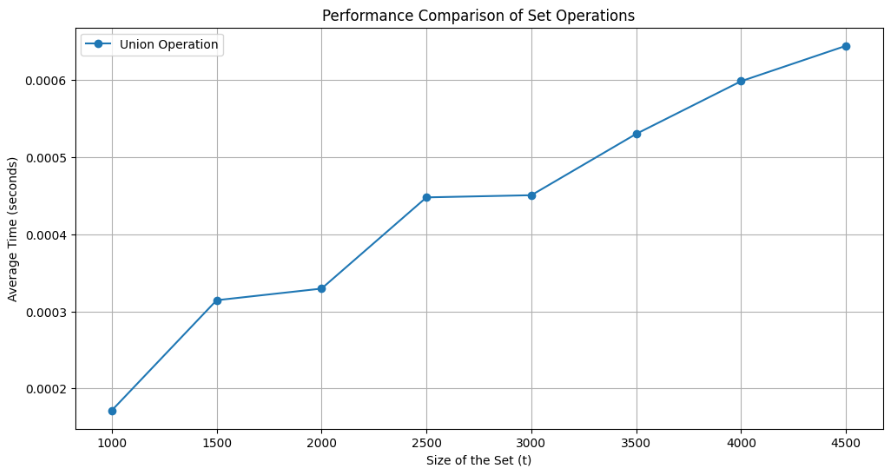
\includegraphics[width=0.8\textwidth]{img/Union.png}
\caption{Порівняння продуктивності операції об'єднання (\texttt{union}) для різних розмірів множин. По горизонтальній осі відкладено розмір множини (\textit{t}), а по вертикальній — середній час виконання операції у секундах.}
\label{fig:union}
\end{figure}

На графіку представлено порівняння продуктивності операції об'єднання (\texttt{union}) для різних розмірів множин. По горизонтальній осі відкладено розмір множини (\textit{t}), а по вертикальній — середній час виконання операції у секундах.

\textbf{Аналіз результатів:} Як видно з графіку, час виконання операції об'єднання поступово зростає зі збільшенням розміру множини. Для невеликих множин (розмір близько 1000 елементів) операція займає приблизно 0.0001 секунди. Однак із збільшенням кількості елементів до 4500 середній час виконання операції підвищується до 0.0007 секунди.

Це свідчить про те, що операція \texttt{union} демонструє лінійну залежність від розміру множини, що можна пояснити її алгоритмічною складністю. Дані підтверджують, що зі зростанням розміру вхідних даних кількість обчислень і, відповідно, час виконання операції зростають майже пропорційно.

\subsection{Результати методу \texttt{search}}
\begin{figure}[h!]
\centering
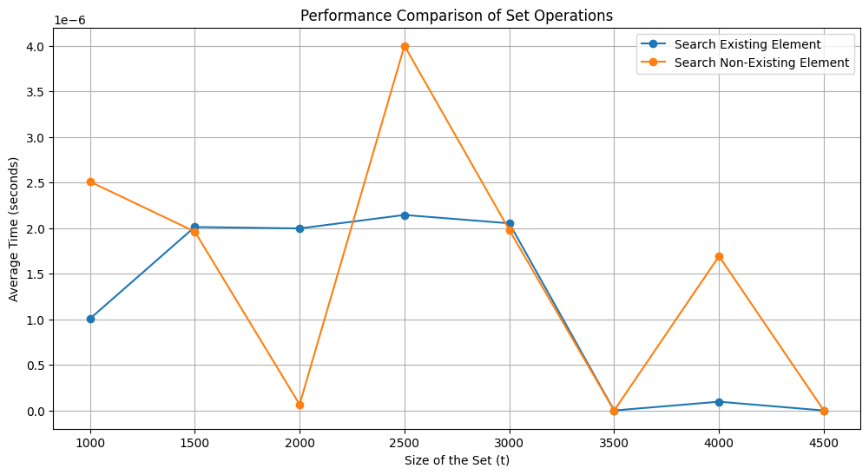
\includegraphics[width=0.8\textwidth]{img/Search.png}
\caption{Порівняння продуктивності операцій пошуку існуючих та неіснуючих елементів у множині різного розміру. По горизонтальній осі відкладено розмір множини (\textit{t}), а по вертикальній — середній час виконання операції у секундах (в масштабі \( e^{-6} \)).}
\label{fig:search}
\end{figure}

\textbf{Аналіз результатів:} Оранжева лінія (пошук неіснуючого елемента) демонструє значні коливання в часі виконання. Наприклад, на множинах розміром близько 2500 елементів спостерігається пікове зростання часу до 4 мікросекунд, після чого час пошуку різко знижується до 0. Це свідчить про непостійний час виконання цієї операції, який може залежати від структури даних, розташування елементів у пам'яті або інших системних факторів.

Синя лінія (пошук існуючого елемента) показує більш стабільну поведінку. На розмірах 1000-3000 час виконання знаходиться в межах 1–2 мікросекунд і має незначні коливання. Після 3000 час падає близько до 0, що може свідчити про оптимізацію або стабільну продуктивність у цих умовах.

\section{Висновки}
Структура, реалізована за допомогою бітових векторів, є ефективною для операцій перевірки наявності, додавання та видалення елементів у множині. Це досягається завдяки константному часу виконання цих операцій.

\end{document}